\subsection{Adversarial Training Theory}\label{sec:adv_theory}
Working with adversarial Neural Networks is quite interesting, as two separate Networks are challenge themselves against each other to improve their performance.
The paper from Goodfellow et. al. \cite{goodfellow2014} describes a game between two Neural Networks (players), where one player has the role of creating fakes and the other must determine if it is real or fake.
The Network who creates fakes is called Generator (G) and the other Network who has to decide about fake or not is called Discriminator (D).
The Generators goal is to create fakes that look like reals, so that D makes mistakes and classifies a fake as a real.
On the other hand the Discriminator is constantly improving itself as well, so that fakes from G can be detected.

This approach works remarkably well as generative network, producing fakes that are astonishing similar to real ones.
In the mentioned paper, this was applied to images and not for audio.
But if the audio waveform is presented as spectogram or mfcc with fixed frame size, it is the same as an image,
where one dimension is time and the other frequency.

So far a generative network does only produce fake images and a discriminative network can only output a one dimensional (probability) output, to decide if it is fake or not.

The idea now is not to use either of these networks, but to use transfer learning in the sense to reuse the convolutional layers both networks achieved during their game, in another network with classification purpose on multiple labels.

\subsubsection{Questions that arise}
There are several questions that arise regarding Adversarial Training:
\begin{enumerate}[label={Q.\textgoth{A}.\arabic*)}, leftmargin=1.4cm]
  \item Do the Network Architectures of G and D have to be the same but transposed?
  \item Does the value space of in and outputs, for D and G respectively, have to be limited e.g. [0, 1] done by e.g. frame normalization, or sigmoid output?
  \item What loss function works well for training?
  \item How long should be trained?
  \item When transfering weights to another network, should the weights from G or D be transfered?
  \item Whats the benefit of all this?
\end{enumerate}

To illustrate the idea an example is shown of the labels L5 (left, right, up, down, go).

The adversarial trained conv layer weights of the individual labels, can be stacked together an used to initialize another network.
An example of this method is shown in \rfig{ml_adv_example}, where the initialzation pattern changes to get more structures and further patterns to be good at classification. However the Basic Pattern from the adversarial training stays the same, which is a good sign, so that the network is able to use this trained weights.

\begin{figure}[!ht]
  \centering
    \subfigure[c1 trained]{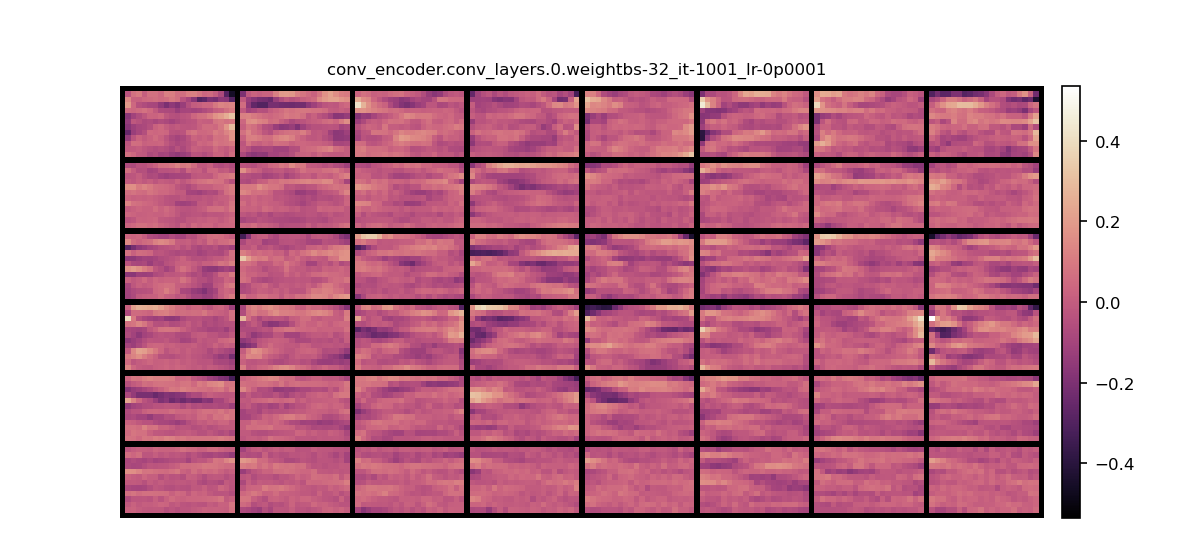
\includegraphics[width=0.45\textwidth]{./3_theory/figs/ml_adv_example_c0}}
    \subfigure[c1 init]{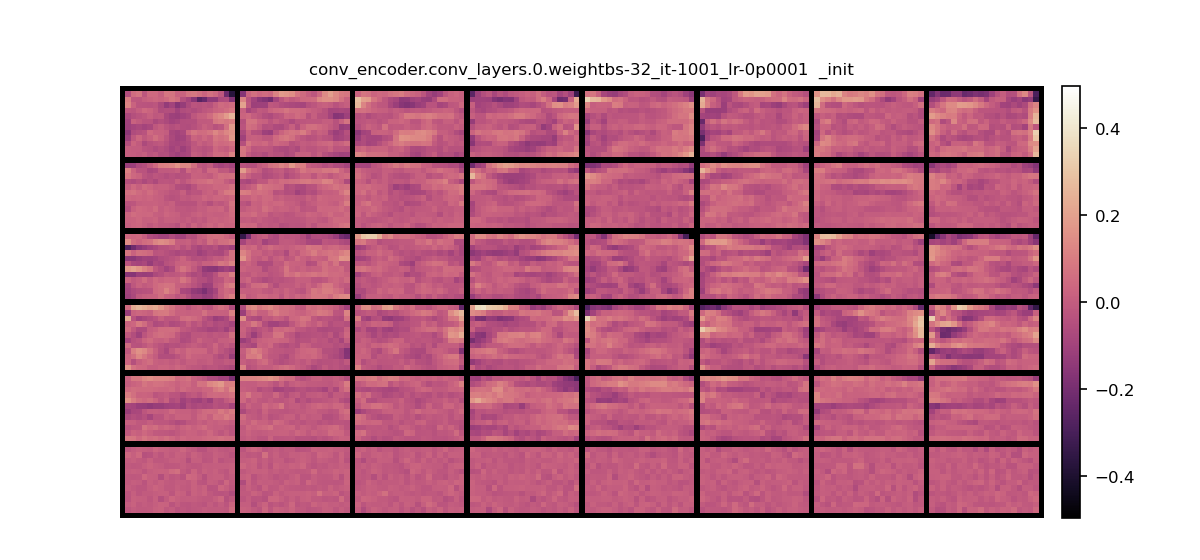
\includegraphics[width=0.45\textwidth]{./3_theory/figs/ml_adv_example_c0_init}}
    \subfigure[c2 trained]{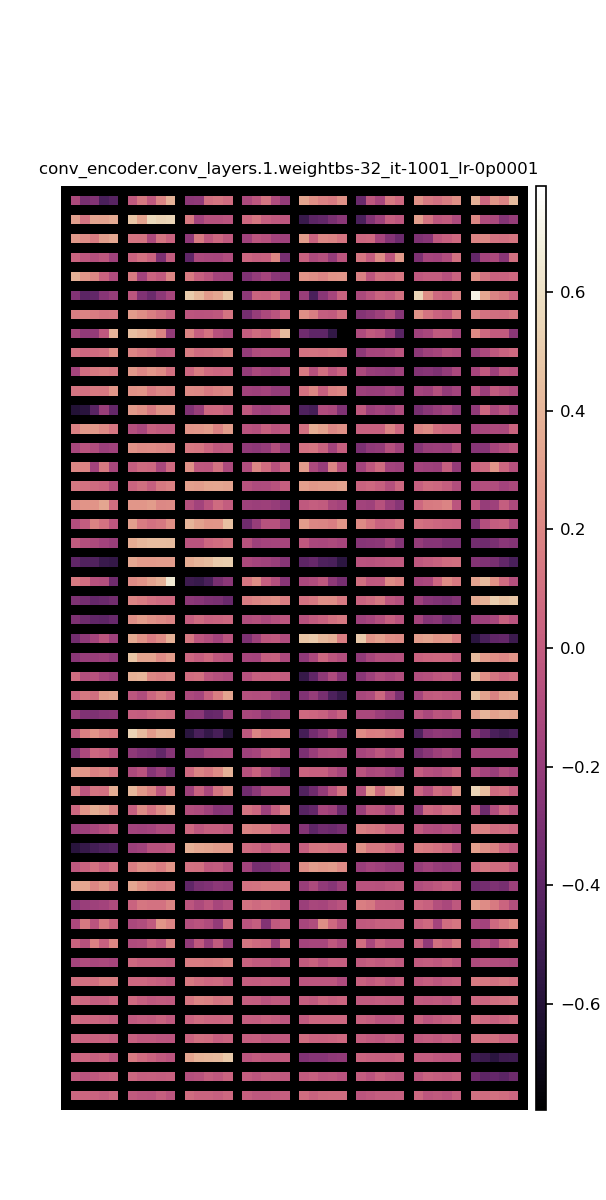
\includegraphics[height=0.45\textwidth]{./3_theory/figs/ml_adv_example_c1}}
    \quad
    \subfigure[c2 init]{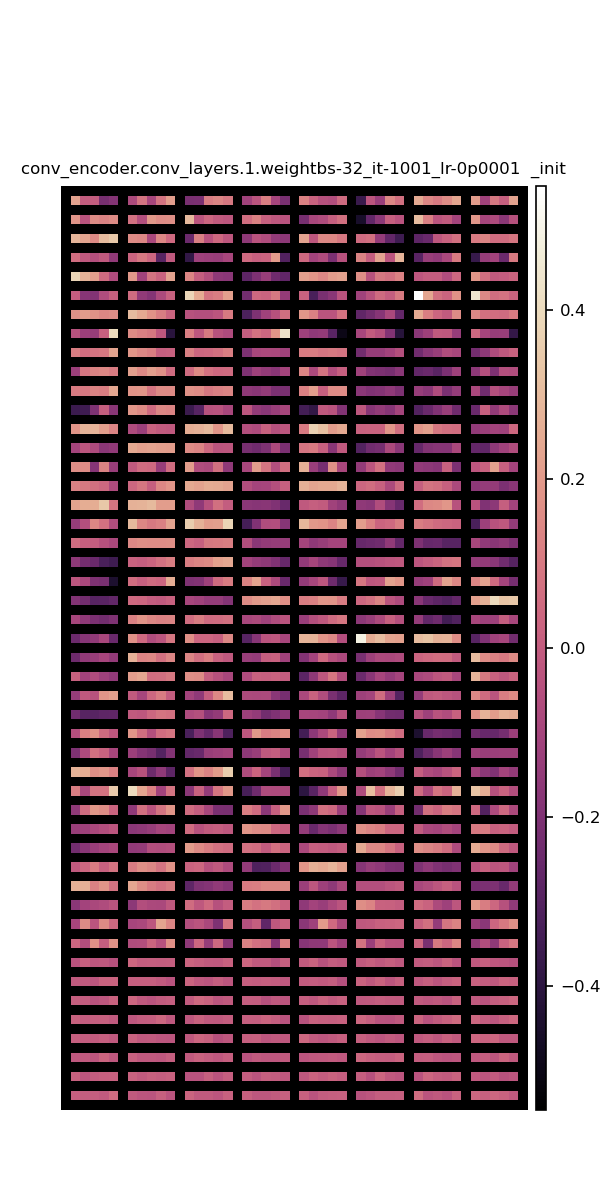
\includegraphics[height=0.45\textwidth]{./3_theory/figs/ml_adv_example_c1_init}}
  \caption{Adversarial Training Example: Convolutional layers pretrained with adversarial training on each label separately.}
  \label{fig:ml_adv_example}
\end{figure}
\FloatBarrier
\noindent

For this example in adversarial training, 8 feature maps of the first layer were used for each label, also they belong to the Generator Network G or decoder (dec). In Convolutional Networks, each previous layers feature map creates a new set of feature maps in the next layer.
An example of this label training is shown in \rfig{ml_adv_example_label} with feature maps [(1, 8), (8, 8)] of the convolutional layers

\begin{figure}[!ht]
  \centering
    \subfigure[left c1 enc]{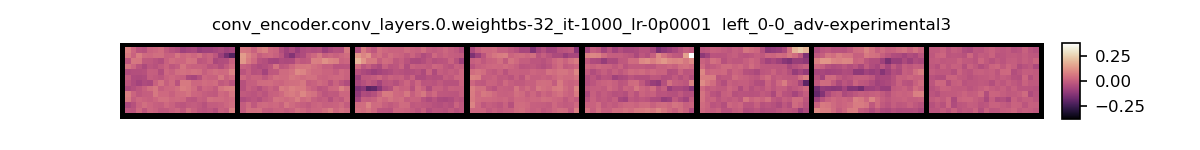
\includegraphics[width=0.45\textwidth]{./3_theory/figs/ml_adv_example_label_left_c0_enc}}
    \subfigure[left c1 dec]{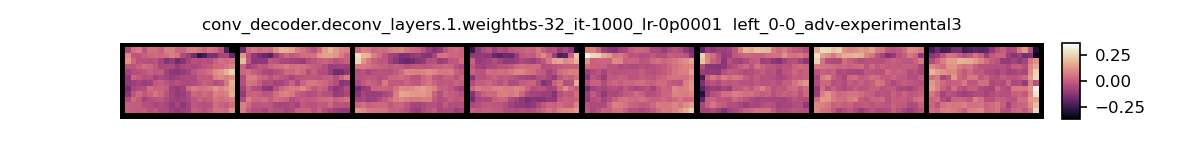
\includegraphics[width=0.45\textwidth]{./3_theory/figs/ml_adv_example_label_left_c0_dec}}
    \subfigure[left c2 enc]{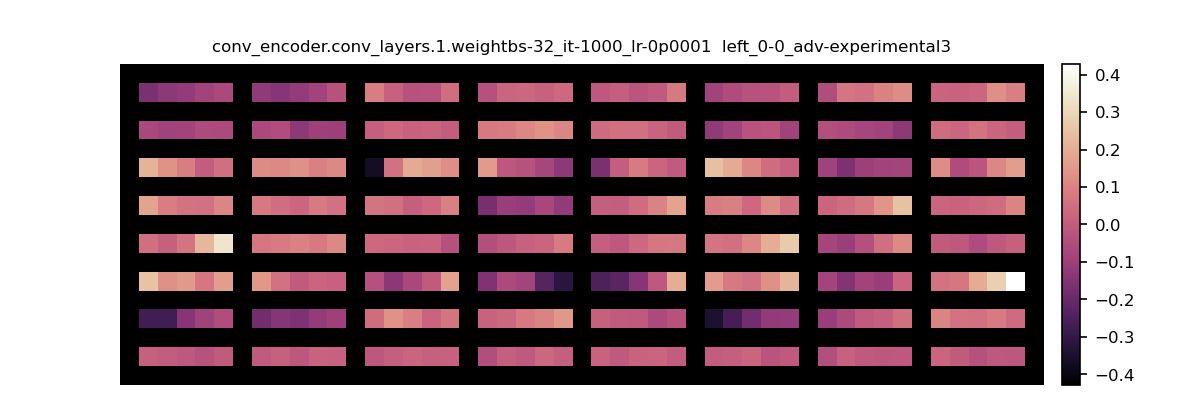
\includegraphics[width=0.45\textwidth]{./3_theory/figs/ml_adv_example_label_left_c1_enc}}
    \subfigure[left c2 dec]{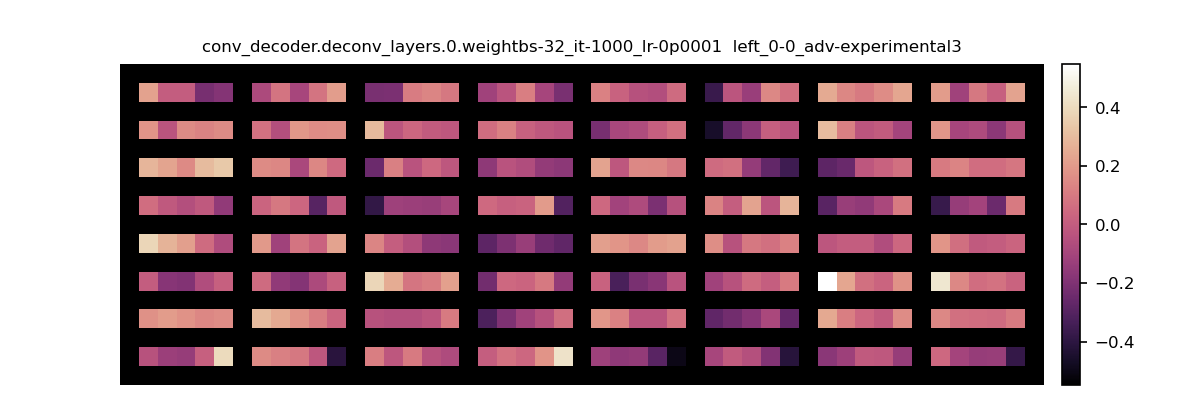
\includegraphics[width=0.45\textwidth]{./3_theory/figs/ml_adv_example_label_left_c1_dec}}
  \caption{Adversarial Training example of label training with label \enquote{left}.}
  \label{fig:ml_adv_example_label}
\end{figure}
\FloatBarrier
\noindent

Those label trained weights can then simply be stacked into the new parameters of a classification network, but it is important that the layers are stacked not randomly, so that the trained connections are still correct.






